To use your Azure Sphere devices with the IoT, you can set up an Azure IoT Hub to work with your Azure Sphere tenant. After you have completed the tasks in this section, any device that is claimed by your Azure Sphere tenant will be automatically enrolled in your IoT hub when it first comes online and connects to the Device Provisioning Service (DPS). Therefore, you only need to complete these steps once.

The following sections will guide you to create an IoT Hub with the Azure Sphere.

\subsection{Step 1: Create an Azure IoT Hub and DPS}
\label{subsec:Step1}
This section shows how to set up the Azure cloud resources in the portal for provisioning your devices.

\subsubsection{Create IoT Hub}
This section describes how to create an IoT hub using the \href{https://portal.azure.com}{Azure Portal}
\begin{enumerate}
    \item Log in to the \href{https://portal.azure.com}{Azure Portal}
    \item Choose \textbf{+Create a resource}, then search for \textbf{IoT Hub}.
    \item Click \textbf{Create} button on the left bottom side of the IoT Hub description.
    \begin{figure}[h]
        \centering
        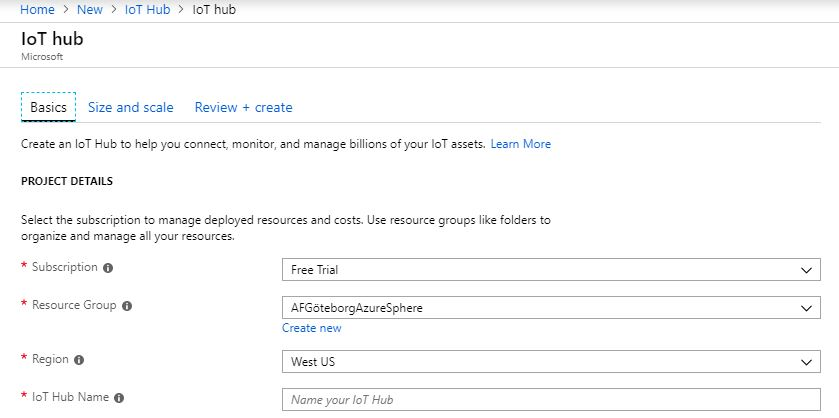
\includegraphics[width=\textwidth]{CreateIoTHub1.JPG}
    \end{figure}
    
    \textbf{Subscription}: Select the subscription to use for your IoT hub.
    
    \textbf{Resource Group}: You can create a new resource group or use an existing one. To create a new one, click Create new and fill in the name you want to use. To use an existing resource group, click Use existing and select the resource group from the dropdown list.
    
    \textbf{Region}: This is the region in which you want your hub to be located. Select the location closest to you from the dropdown list.

    \textbf{IoT Hub Name}: Put in the name for your IoT Hub. This name must be globally unique. If the name you enter is available, a green check mark appears. 
    \newpage
    \item Click \textbf{Next: Size and scale} to continue creating your IoT hub.
    \begin{figure}[h]
        \centering
        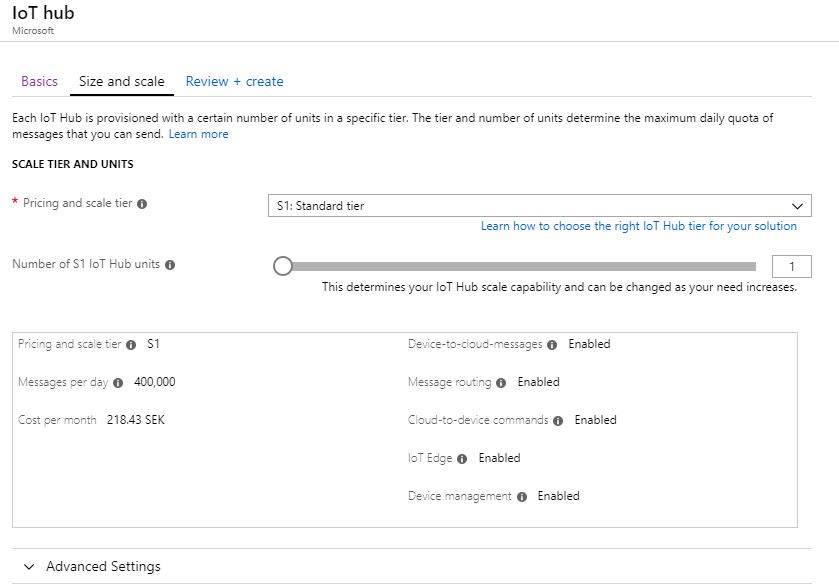
\includegraphics[width=\textwidth]{CreateIoTHub2.JPG}
    \end{figure}
    
    On this screen, you can take the defaults and just click Review + create at the bottom.
    
    \textbf{Pricing and scale tier}: You can choose from several tiers depending on how many features you want and how many messages you send through your solution per day. The free tier is intended for testing and evaluation. It allows 500 devices to be connected to the IoT hub and up to 8,000 messages per day. Each Azure subscription can create one IoT Hub in the free tier.

    \textbf{IoT Hub units}: The number of messages allowed per unit per day depends on your hub's pricing tier. For example, if you want the IoT hub to support ingress of 700,000 messages, you choose two S1 tier units.
    
    \textbf{Advanced / Device-to-cloud partitions}: This property relates the device-to-cloud messages to the number of simultaneous readers of the messages. Most IoT hubs only need four partitions.
    
    \item Click Review + create to review your choices. You should see the similar screen as:
    \begin{figure}[h]
        \centering
        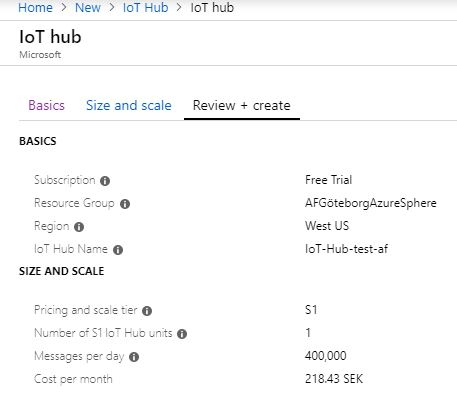
\includegraphics[scale=0.55]{CreateIoTHub3.JPG}
    \end{figure}
    
    \item Click Create to create your new IoT hub. Creating the hub takes a few minutes.
    
    \item In our condition, the IoT Hub has already been created as "azure-temperature-hub", but you can create a new one.
\end{enumerate}


\subsubsection{Create IoT Hub Device Provisioning Service}
\begin{enumerate}
    \item Click the \textbf{Create a resource} button and searching for the \textbf{IoT Hub Device Provisioning Service}. Then click \textbf{Create}
    \item Filling the following information for your new Device Provisioning service and click \textbf{Create}.
          \begin{itemize}
              \item \textbf{Name}: Provide a unique name of the instance. If the name is available, a green check mark appears in the end.
              \item \textbf{Subscription}: Choose the subscription that you want to use to create this Device Provisioning service instance.
              \item \textbf{Resource Group}: You can create a new resource group in this field, or choosing an existing one. 
              \item \textbf{Location}: Select the location to your device.
          \end{itemize}
          \begin{figure}
            \centering
            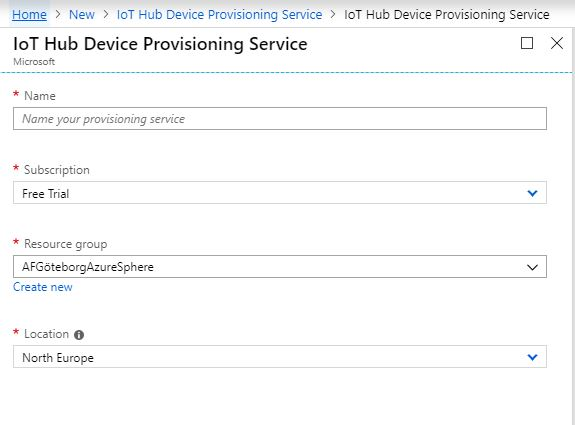
\includegraphics[scale=0.45]{DeviceProvisioningService.JPG}
          \end{figure}
    \item Once the service is successfully deployed, the notifications will notify you, then click \textbf{Go to resource}
    \item In our condition, the name of the provision is "afgoteborg-azure-provision"
\end{enumerate}

\subsubsection{Link the IoT Hub and Device Provisioning Service}
This section describes the configuration in the Device Provisioning Service sets the IoT hub for the devices will be provisioned.
\begin{enumerate}
    \item Click the \textbf{All resources} button from the left-hand menu of the Azure portal. Select the Device Provisioning service that you created in the preceding section.
    \item Under the settings, select Linked IoT hubs. Then click \textbf{+Add}. 
    \item In the \textbf{Add link to IoT hub}, provide the following information to link your new Device Provisioning service instance to an IoT hub. Then click Save.
          \begin{itemize}
              \item \textbf{Subscription}: Select the subscription containing the IoT hub that you want to link with your new Device Provisioning service instance.
              \item \textbf{Iot hub}: Select the IoT hub to link with your new Device Provisioning service instance.
              \item \textbf{Access Policy}: Select iothubowner as the credentials for establishing the link with the IoT hub.
          \end{itemize}
          \begin{figure}
            \centering
            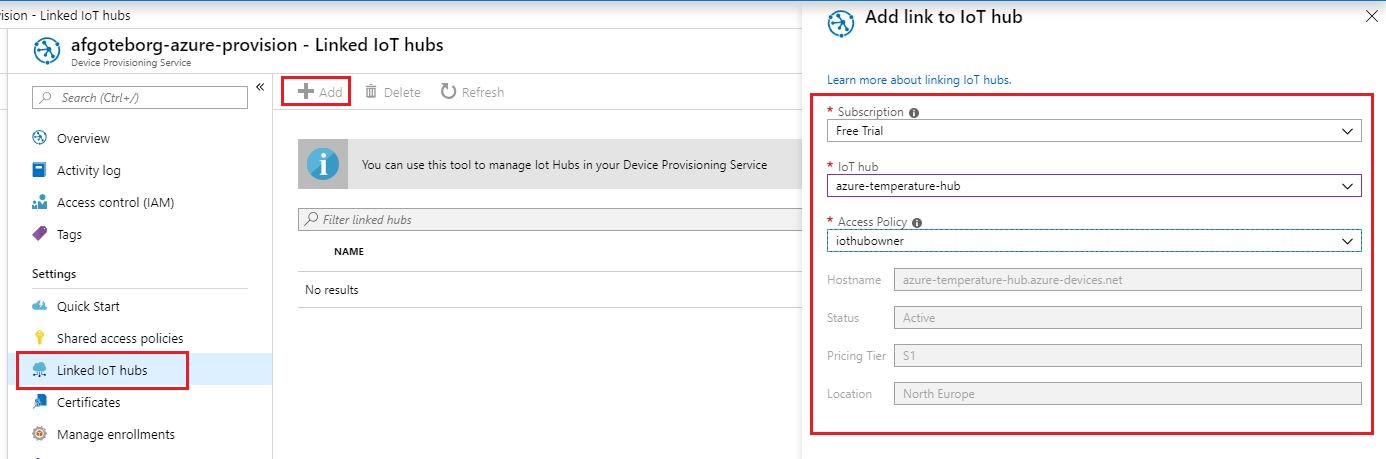
\includegraphics[width=\textwidth]{LinkIoT.JPG}
      \end{figure}
      \item You should be able to see the newly created Linked IoT hubs in the list.
\end{enumerate}

\subsubsection{Clean up resources}
If you want to continue on this tutorial, you do not need to do this step. If you are not, use the following steps to delete the resources just created.
\begin{enumerate}
    \item From the left-hand menu in the Azure portal, click \textbf{All resources} and then select your Device Provisioning service. At the top of the \textbf{All resources} blade, click \textbf{Delete}.
    \item From the left-hand menu in the Azure portal, click \textbf{All resources} and then select your IoT hub. At the top of the All resources blade, click \textbf{Delete}.
\end{enumerate}

\subsection{Step2: Download the tenant authentication}
After finished the previous section, we can set up the Azure Sphere device with the IoT.
\begin{enumerate}
    \item Open the Azure Sphere Developer Command Prompt in the Start menu.
    \item Sign in with the user for your Azure Active Directory:
    \begin{lstlisting}[language=bash]
        azsphere login
    \end{lstlisting}
    \item Download the Certificate Authority (CA) certificate for your Azure Sphere tenant, the output file must have the .cer extension.
    \begin{lstlisting}[language=bash]
        azsphere tenant download-CA-certificate --output AFTechCert.cer
    \end{lstlisting}
\end{enumerate}

\subsection{Step3: Upload the tenant CA certificate to DPS and generate a verification code}
\begin{enumerate}
    \item Log in to the \href{https://portal.azure.com}{Azure Portal} and navigate to the  DPS(Device Provisioning Service) you created in \ref{subsec:Step1}
    \item Open \textbf{Certificates} from the menu. 
    \begin{figure}[h]
        \centering
        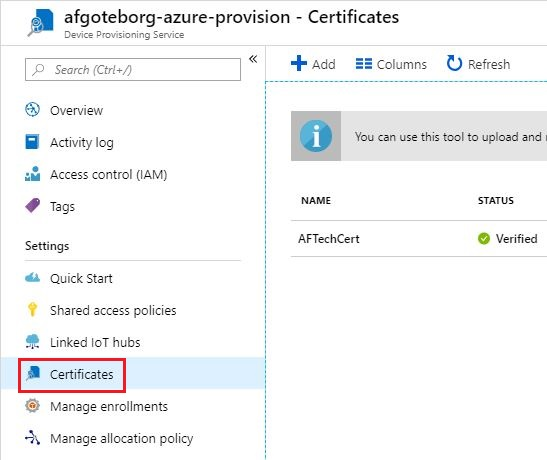
\includegraphics[scale=0.6]{DPSCert.JPG}
    \end{figure}
    \newpage
    \item Then click \textbf{ADD} to add a new certificate and enter a name for your certificate. Upload the .cer file from Step 2.
    \begin{figure}[h]
        \centering
        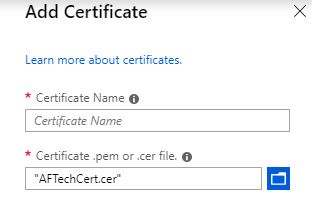
\includegraphics[scale=0.7]{DPSAddCert.JPG}
    \end{figure}
    \item After you are notified that the certificate uploaded successfully, click \textbf{Save}.
    \item The new certificate is listed under the explorer. Note the STATUS of the certificate is Unverified. Click on this certificate.
    \begin{figure}[h]
        \centering
        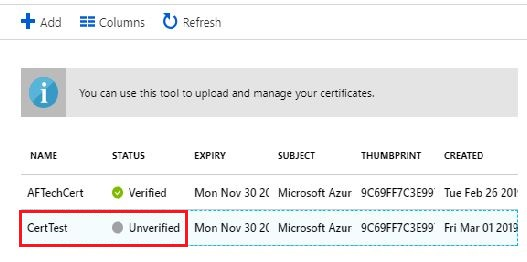
\includegraphics[scale=0.7]{DSPCertUnVer.JPG}
    \end{figure}
    \item In \textbf{Certificate Details}, click Generate Verification Code. The DPS creates a Verification Code that you can use to validate the certificate ownership. Copy the code to your clipboard for use in the next step.
    
\end{enumerate}

\subsection{Step 4: Verify the tenant CA certificate}
\begin{enumerate}
    \item Back to the Azure Sphere Developer Command Prompt. Download the validation certificate based on your own tenant CA certificate. Replace code in the command with the verification code from the previous setp.
    \begin{lstlisting}[language=bash]
        azsphere tenant download-validation-certificate --output AFTechValidationCert.cer --verificationcode <code>
    \end{lstlisting}
    The Azure Sphere Security Service signs the validation certificate with the verification code from the DPS to your own CA.
    \item Return to the Azure Portal to upload the validation certificate to DPS. In \textbf{Certificate Details}, use the File Explorer icon next to the \textbf{Verification Certificate .pem or .cer file} field to upload the signed verification certificate. Then click \textbf{Verify}.
     \begin{minipage}{.45\textwidth}
        \centering
        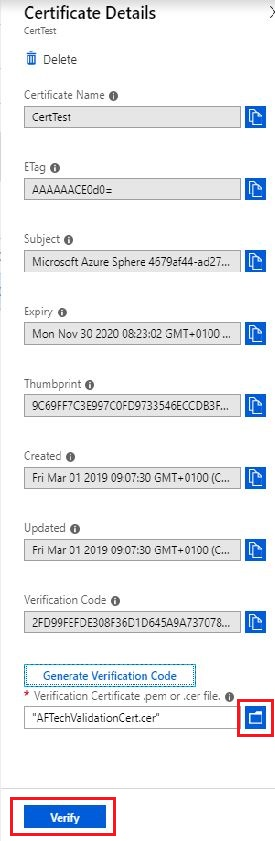
\includegraphics[scale=0.8]{CertificatDetails.JPG}
    \end{minipage}
    \item The \textbf{STATUS} of the certificate changes to \textbf{Verified} in the list. Click \textbf{Refresh} if it does not update automatically.
\end{enumerate}
\newpage
\subsection{Step 5: Use the certification to add you device to and enrollment group}
\begin{enumerate}
    \item In the same DPS view as previous step. Select \textbf{Manage enrollment}, then click \textbf{Add enrollment group}.
    \item In the Add Enrollment Group panel, create a name for your enrollment group, select CA Certificate as the \textbf{Certificate type}, and select the certificate that you validated in the previous step.
    \item Click \textbf{Save}. You should see the group name appears under the \textbf{Enrollment Group} on the successful creation of the enrollment group.
    \begin{figure}[h]
        \centering
        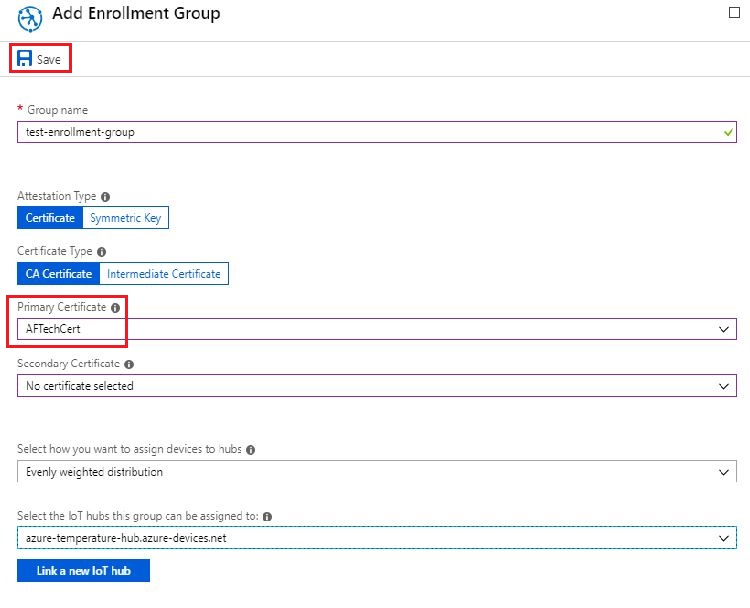
\includegraphics[scale=0.5]{EnrollmentGroup.JPG}
    \end{figure}
\end{enumerate}

\subsection{Azure Sphere IoT Hub Sample Application}
The Azure IoT Hub sample application shows the communication between the Azure IoT Hub and the Azure Sphere Device.

This sample uses the Connected Service for Azure Sphere, which is installed with the Azure Sphere SDK. The Visual Studio provides a template for connecting
the Azure Sphere device to your IoT hub and communication with the hub. Application that use the Connected Service functionality can send messages to and 
receive messages from and IoT Hub, maintain a device twin, and direct method calls from cloud service.

This sample does the following:
\begin{enumerate}
    \item Displays the currently connected WiFi network
    \item Blinks LED 1 constantly. Pressing button A changes the rate. The rate is also stored in the device twin so that a cloud service program can change it.
    \item Sends a message to the IoT Hub when you press button B.
    \item Lights LED 3 green after start-up to indicate that the device has connected to the IoT Hub and the application has successfully authenticated with the hub.
    \item Changes the color of LED 1 in response to a direct method call.
\end{enumerate}

You must set up the board:
\begin{enumerate}
    \item Connect to a PC and to WiFi network.
    \item Change the board to prep-debug.
\end{enumerate}

\subsubsection{Add the device to the IoT hub}
\begin{enumerate}
    \item Start Visual Studio 2017 and go to \textbf{File>New>Project}. Navigate to the template in \textbf{Visual C++>Cross Platform>Azure Sphere}. Select Azure IoT Hub Sample for MT3620 RDB (Azure Sphere), specify a name and location or use the defaults, and select OK.
    \item In Solution Explorer, right click on \textbf{Reference} and then select \textbf{Add Connected Service}
    \begin{figure}[h]
        \centering
        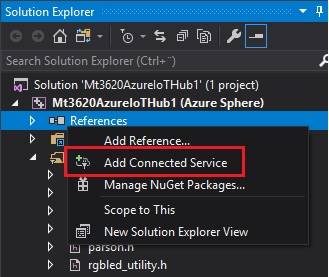
\includegraphics[scale=0.6]{VSAddConnectService.jpg}
    \end{figure}
    \item Select \textbf{Device Connectivity with Azure IoT} from the list of connected services.
    \begin{figure}[h]
        \centering
        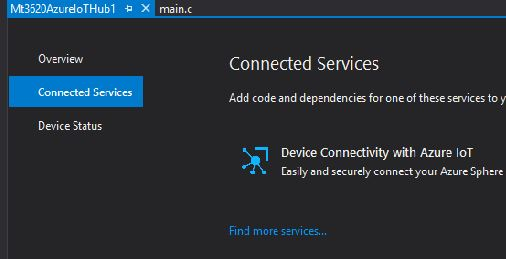
\includegraphics[scale=0.5]{AddConServiecPan.JPG}
    \end{figure}
    \item It may ask you to log in to the account you're using with your Azure Sphere tenant.
    \item In the Device Connectivity, select your Azure subscription from the \textbf{Subscription} dropdown. Select Device Provisioning Service from the \textbf{Connection Type} dropdown. Select your Device Provisioning Service from the \textbf{Device Provisioning Service} dropdown.
    \begin{figure}[h]
        \centering
        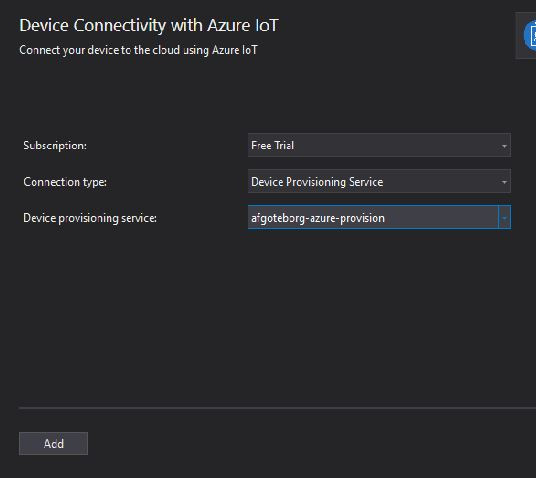
\includegraphics[scale=0.5]{CreateDiveConIoT.JPG}
    \end{figure}
    \item Click Add.
    \item In Solution Explorer, you should now see azure\_iot\_utilities.h and azure\_iot\_utilities.c in your solution. In addition, the host name for the Azure IoT Hub has been added to the Capabilities section of the app\_manifest.json file. An application can connect only to the internet hosts that are specified in the AllowedConnections field.
    \begin{figure}[h]
        \centering
        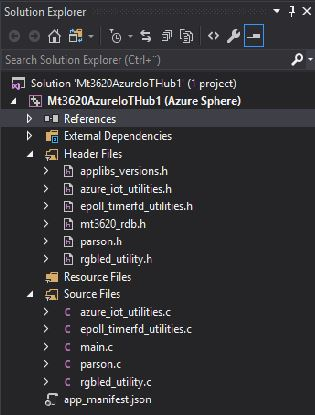
\includegraphics[scale=0.55]{IoTSolutionExplorer.JPG}
    \end{figure}
\end{enumerate}

\subsubsection{Start the Sample}
\begin{enumerate}
    \item Open main.c in the sample application
    \item Press F5 to build, load and start the sample.
    
    The sample opens the handles to the buttons and the RGB LEDs, it also displays the connected WiFi network.

    Then it starts the main loop. You should see LED 1 start to blink and see output like the following in the Output window:
    \begin{figure}[h]
        \centering
        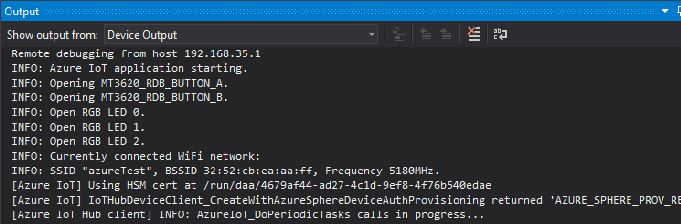
\includegraphics[scale=0.7]{ASIoTOutput.JPG}
    \end{figure}
\end{enumerate} 

\subsubsection{Send and receive messages}
In Azure Portal you can send and receive the messages from your device.
\begin{enumerate}
    \item Log in to Azure Portal with the IoT Hub we created previously.
    \item Select \textbf{All Resources} on the left panel. Click on the IoT hub in the resource list.
    \item Navigate to \textbf{IoT devices} in the Explorers section in the IoT Hub panel. You may need to scroll down a little bit.
    \begin{figure}[h]
        \centering
        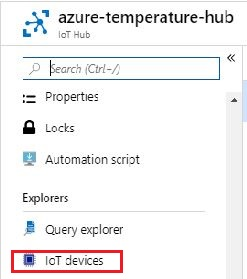
\includegraphics[scale=0.65]{SelectIoTDevice.JPG}
    \end{figure}
    \item You should see the device id in the list. Click on the device id to open the \textbf{Device details} panel.
    \item Click on the \textbf{Message to device}. In the \textbf{Message to device} type some messages, for example "Hello from Portal" in the \textbf{Message Body} textbox. Then click \textbf{Send Message}.
    \begin{figure}[h]
        \centering
        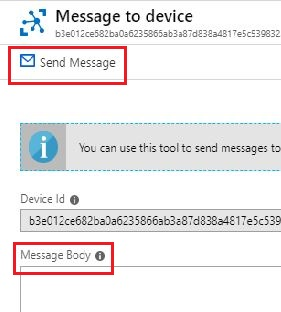
\includegraphics[scale=0.6]{MsgToDevice.JPG}
    \end{figure}
    Back to Visual Studio 2017, in the output Windows you should see a message \textbf{[Azure IoT] INFO: Received message 'Hello from Portal' from IoT Hub} coming out in the output windows.
\end{enumerate}

\subsubsection{Call a direct method on the device}
\begin{enumerate}
    \item Back to Device Details in the portal. You may see the prompt said "Your unsaved edit will be discarded", click \textbf{OK}. Then select \textbf{Direct method}.
    \item In the \textbf{Direct method} panel, fill in \textbf{LedColorControlMethod} under the \textbf{Method Name} box, and \textbf{{"color":"green"}} in the Method payload box. Then click \textbf{Invode Method}.
    \begin{figure}[h]
        \centering
        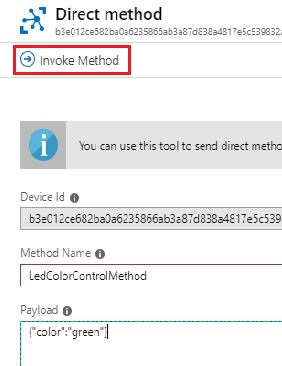
\includegraphics[scale=0.7]{DirectMethod.JPG}
    \end{figure}
    \item You should see the following output in the Visual Studio output window and LED 1 start blinking green.
    \begin{lstlisting}[language=bash]
    [Azure IoT] INFO: Trying to invoke method LedColorControlMethod
    INFO: LED color set to: 'green'.
    \end{lstlisting}
    In the meantime, check the Result in the Direct Method in the portal, the return payload should be 
    \begin{lstlisting}[language=bash]
    {"success":true,"message":"led color set to green"}
    \end{lstlisting}
\end{enumerate}

\subsubsection{Manage a device twin}
A device twin is a JSON document in the cloud that stores information about a device. Use the device twin to synchronize status information and maintain device properties that should be accessible to cloud service applications as well as to applications that run on the device.
\begin{enumerate}
    \item Back to Device Details in the portal. Then select \textbf{Device twin}.
    \item You should see the JSON document in the panel. Find \textbf{LedBlinkRateProperty} under \textbf{desired} properties, if you cannot find it, please add it before \textbf{metadata}. Set the value 0, 1 or 2.
    \item Then click \textbf{Save}.
    \begin{figure}[h]
        \centering
        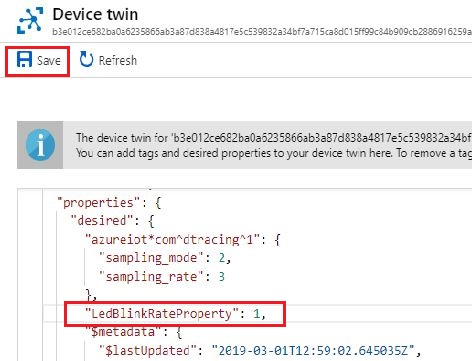
\includegraphics[scale=0.7]{DeviceTwin.JPG}
    \end{figure}
    \item In Visual Studio, check the Output window. You should see:
    \begin{lstlisting}[language=bash]
    INFO: Received desired value 1 for LedBlinkRateProperty, setting it to 1.
    [Azure IoT] INFO: Set reported property 'LedBlinkRateProperty' to value 1.
    \end{lstlisting}
    In the meantime, the blinking rate of the LED 1 should be changed.
\end{enumerate}